\section{Exploratory data analysis}
\tbl{summary_statistics.tex}

\subsection{Temperature}
Figure~\ref{fig:tempdist} shows that Africa and Oceania (mostly tropical capitals) are warm with narrow
distributions. Europe and Asia span more than 40\,\textdegree C over the year. The monthly curves
(Figure~\ref{fig:monthly}) show the two hemispheres in opposite phase, with Europe swinging the most.

\begin{figure}[H]\centering
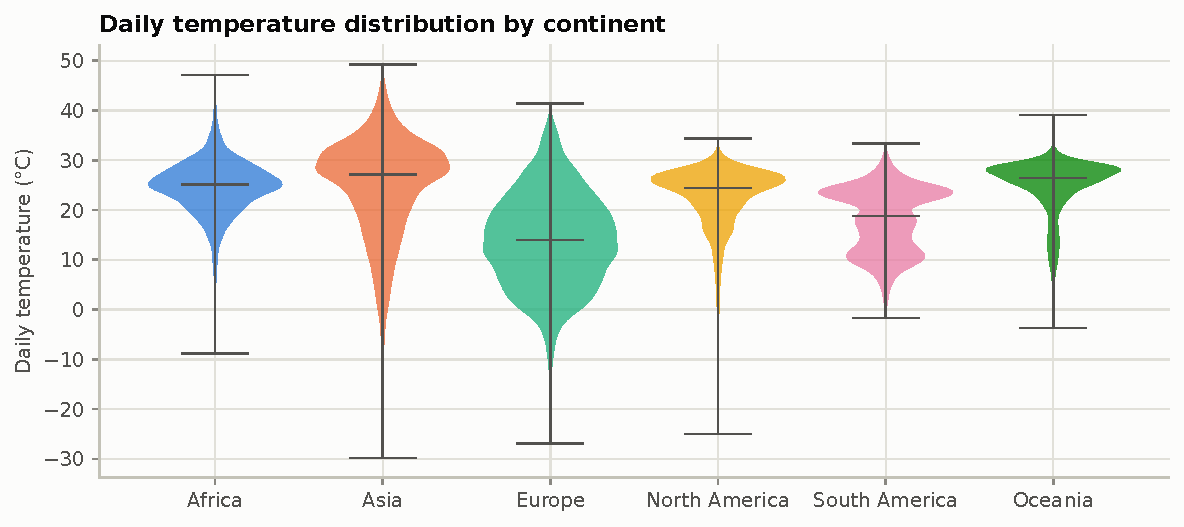
\includegraphics[width=0.85\linewidth]{eda/temperature_distribution_by_continent}
\caption{Daily temperature by continent.}\label{fig:tempdist}
\end{figure}
\begin{figure}[H]\centering
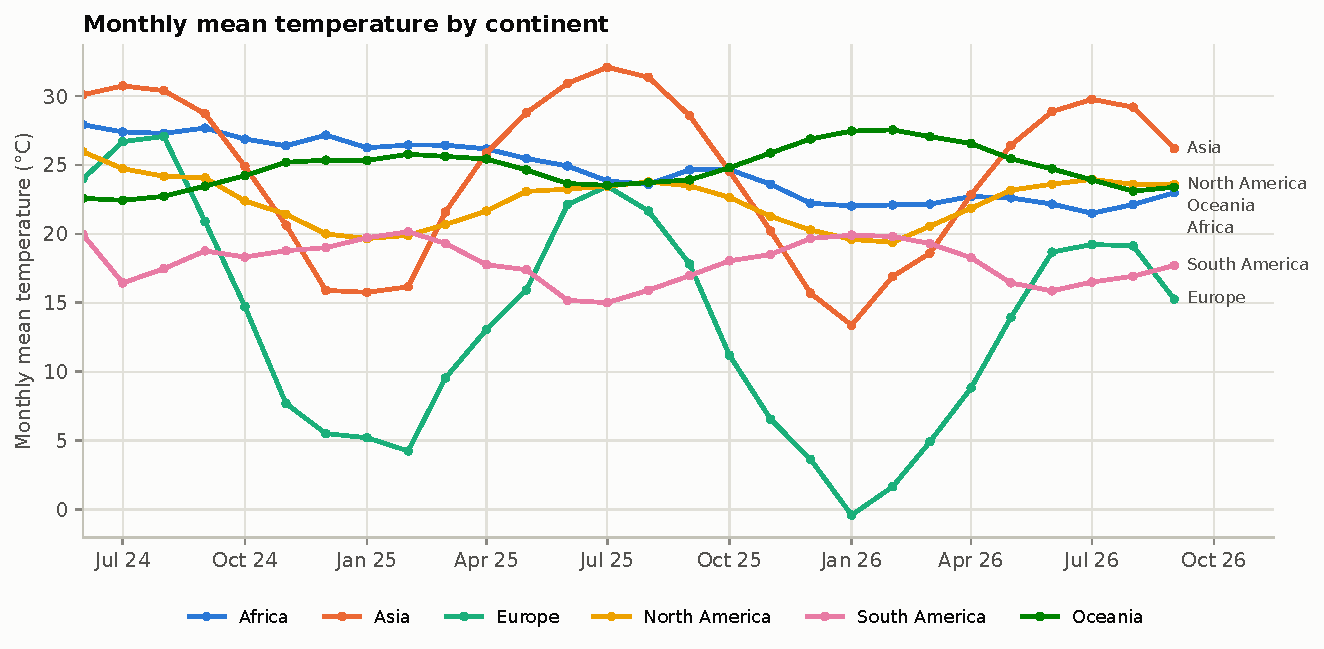
\includegraphics[width=0.9\linewidth]{eda/monthly_temperature_by_continent}
\caption{Monthly mean temperature per continent (partial first and last months removed).}\label{fig:monthly}
\end{figure}

\subsection{A hidden confounder: the snapshot hour}\label{sec:hour}
The global mean temperature of the 184 well-covered capitals (Figure~\ref{fig:global}) appears to cool
sharply. The cause is the \emph{local clock time of the snapshot}. Its median drifts from 16:30 in mid-2024
to 07:45 in late 2026 (Figure~\ref{fig:hour}), so recent observations are increasingly taken near the daily
minimum. We regress the series on a linear trend, three annual harmonics and the mean diurnal harmonics
(Figure~\ref{fig:decomp}). This shrinks the apparent trend from \textbf{$-1.80$} to
\textbf{$-0.26$\,\textdegree C/yr}, leaving an annual cycle with an amplitude of about 9.4\,\textdegree C.
Without this correction, any trend model would mistake a change in sampling for climate change.

\begin{figure}[H]\centering
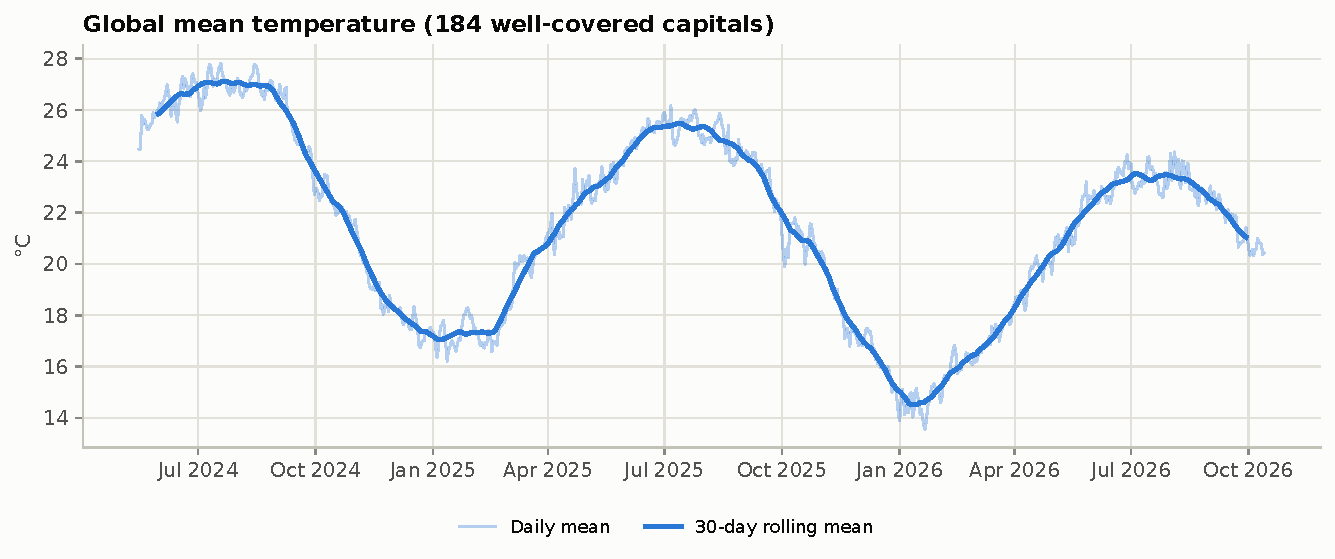
\includegraphics[width=0.9\linewidth]{eda/global_temperature_trend}
\caption{Global mean temperature, daily and 30-day rolling mean.}\label{fig:global}
\end{figure}
\begin{figure}[H]\centering
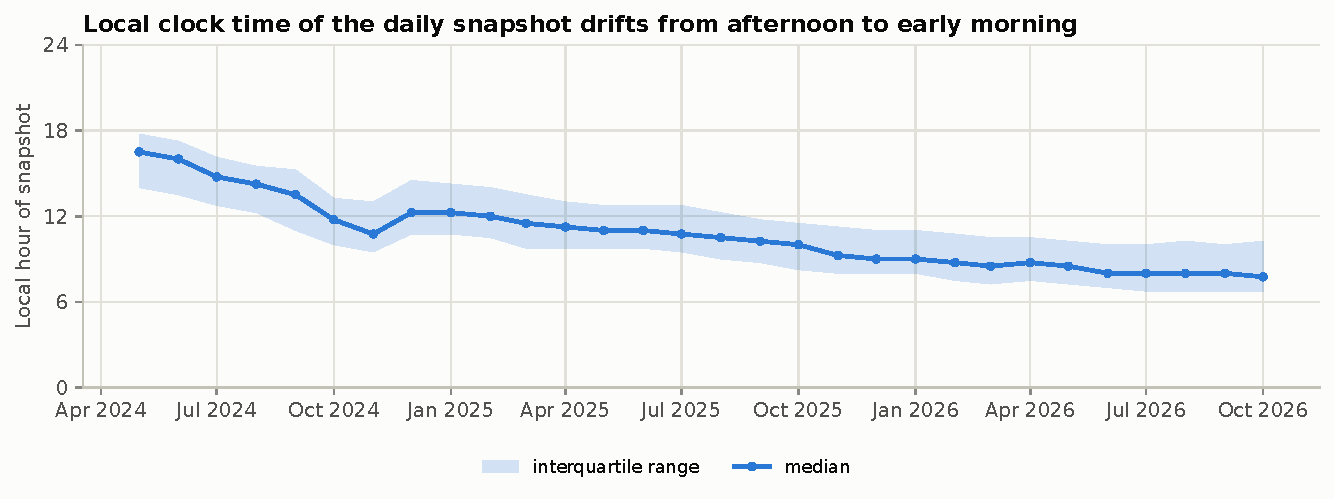
\includegraphics[width=0.9\linewidth]{eda/observation_hour_drift}
\caption{Local hour of the daily snapshot (median and IQR across cities).}\label{fig:hour}
\end{figure}
\begin{figure}[H]\centering
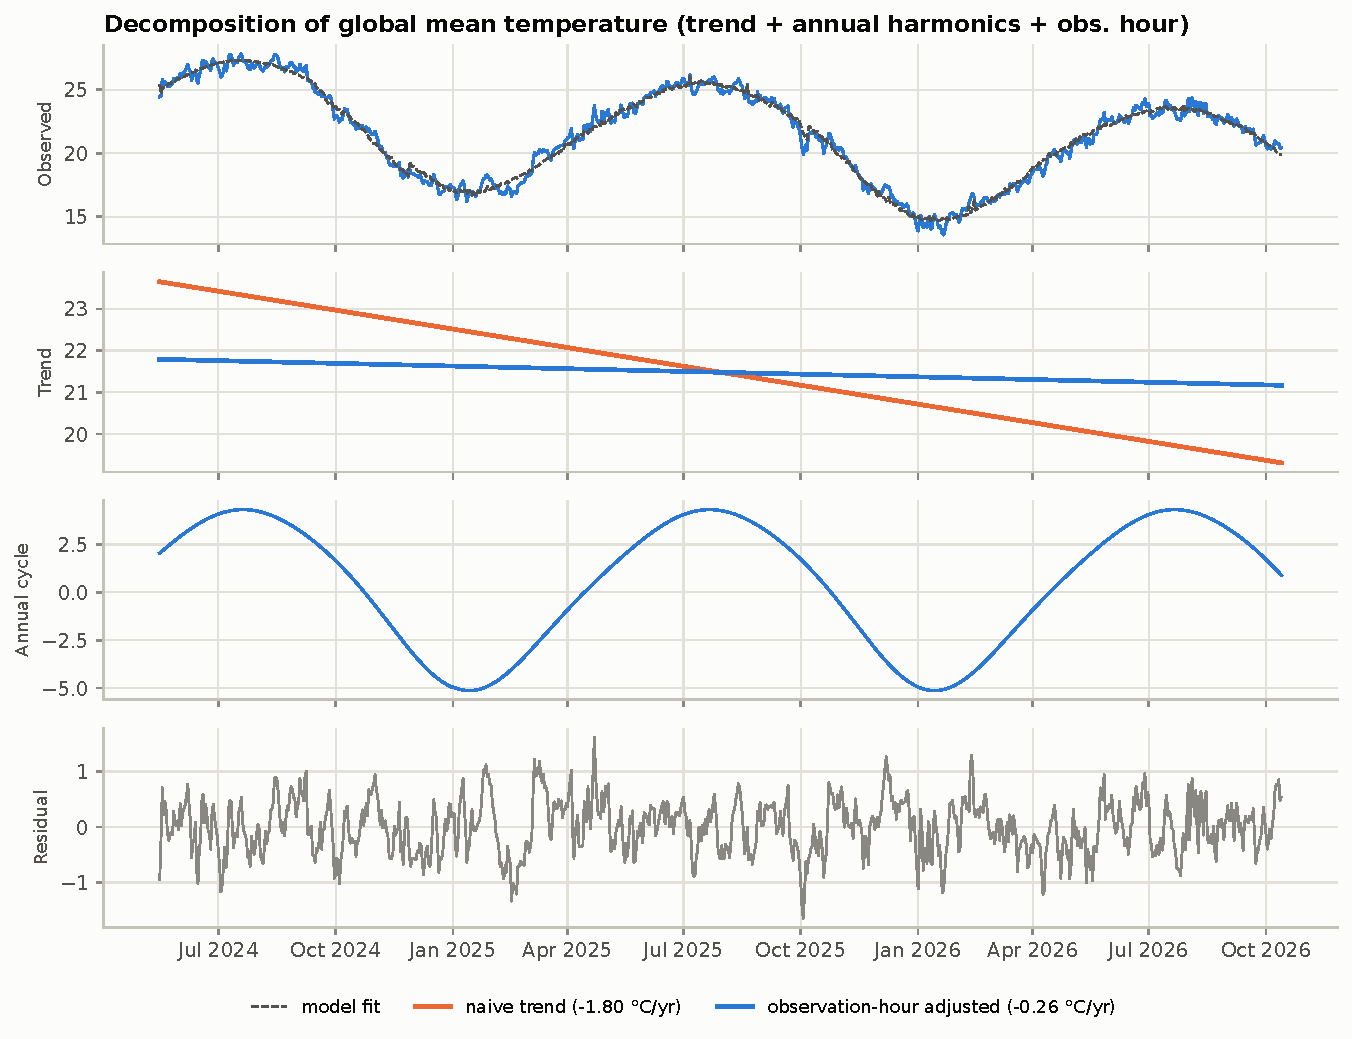
\includegraphics[width=0.9\linewidth]{eda/global_temperature_decomposition}
\caption{Harmonic-regression decomposition of global mean temperature. STL is degenerate with only about 2.4
annual cycles, so it is not used.}\label{fig:decomp}
\end{figure}

\subsection{Precipitation}
Precipitation is zero-inflated: 67\,\% of snapshots record no rain, and wet-day amounts are roughly
log-normal (Figure~\ref{fig:precip}). Seasonality differs by region (Figure~\ref{fig:precipheat}). Asia and
Oceania peak in the boreal-summer monsoon, while South America and Africa follow the migration of the ITCZ.

\begin{figure}[H]\centering
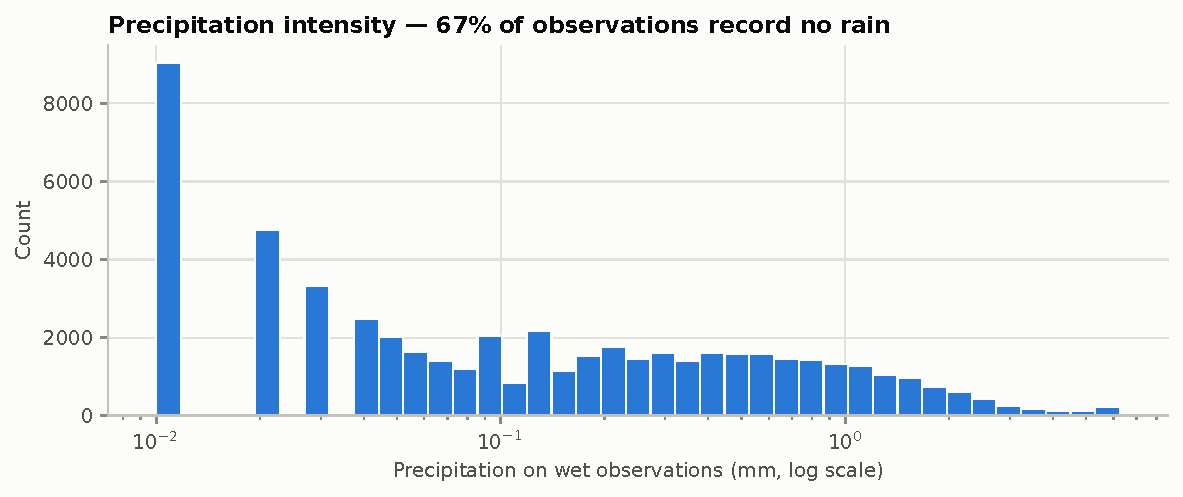
\includegraphics[width=0.8\linewidth]{eda/precipitation_distribution}
\caption{Wet-observation precipitation intensity (log scale).}\label{fig:precip}
\end{figure}
\begin{figure}[H]\centering
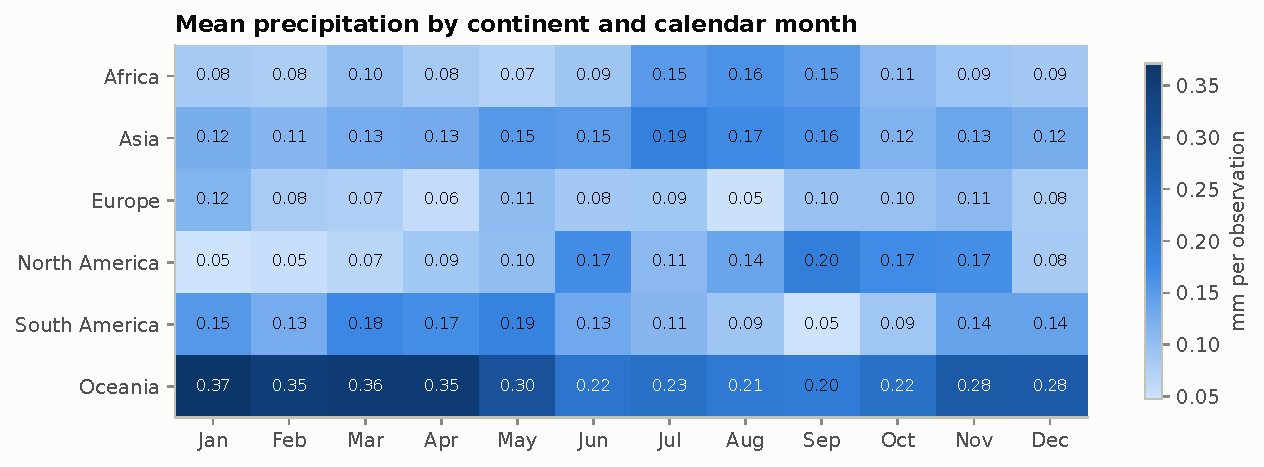
\includegraphics[width=0.9\linewidth]{eda/precipitation_heatmap_continent_month}
\caption{Mean precipitation by continent and calendar month.}\label{fig:precipheat}
\end{figure}
\begin{figure}[H]\centering
\begin{subfigure}{0.49\linewidth}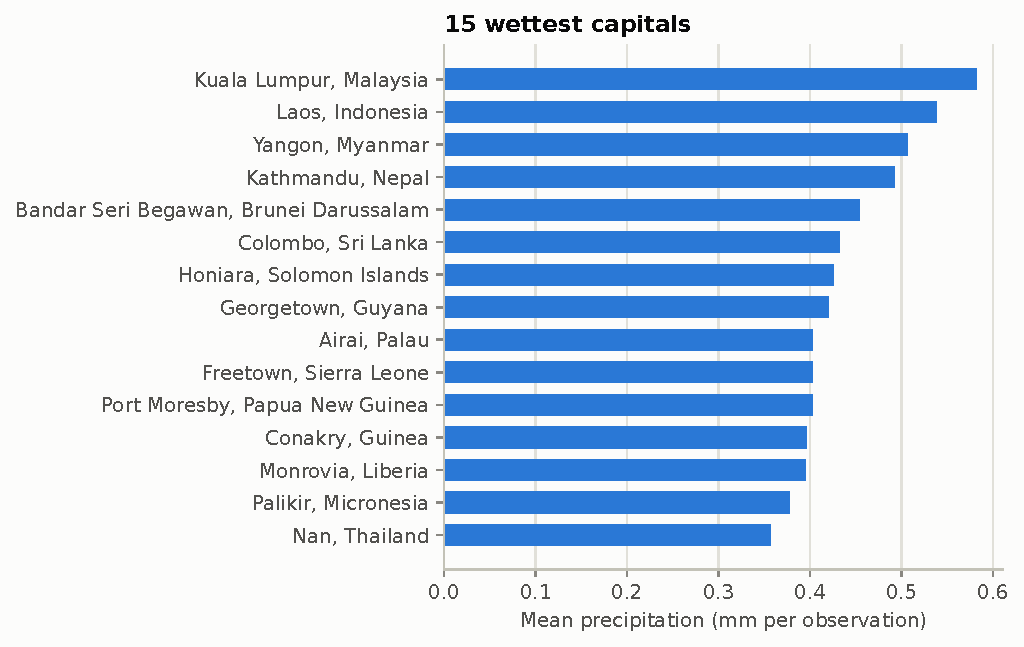
\includegraphics[width=\linewidth]{eda/wettest_capitals}\end{subfigure}
\begin{subfigure}{0.49\linewidth}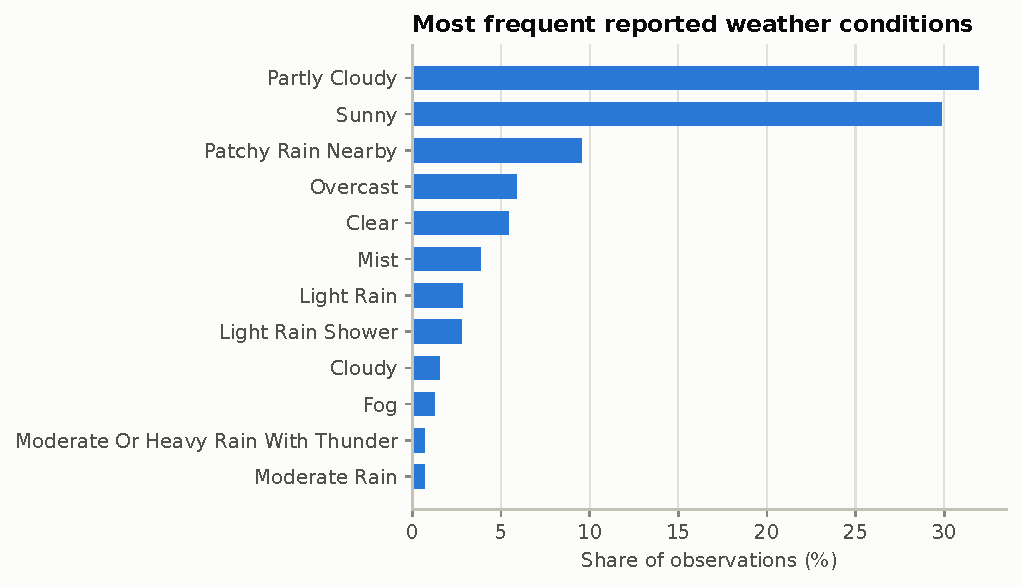
\includegraphics[width=\linewidth]{eda/weather_conditions}\end{subfigure}
\caption{Wettest capitals (left) and most frequent reported conditions (right).}
\end{figure}

\subsection{Correlations}
Spearman correlations (Figure~\ref{fig:corr}) match physical expectations:
\begin{itemize}
  \item temperature tracks feels-like and UV ($\rho\approx0.44$);
  \item humidity is anti-correlated with temperature ($\rho\approx-0.32$) and with visibility;
  \item PM2.5 and PM10 are almost collinear;
  \item ozone rises with UV and falls with humidity.
\end{itemize}

\begin{figure}[H]\centering
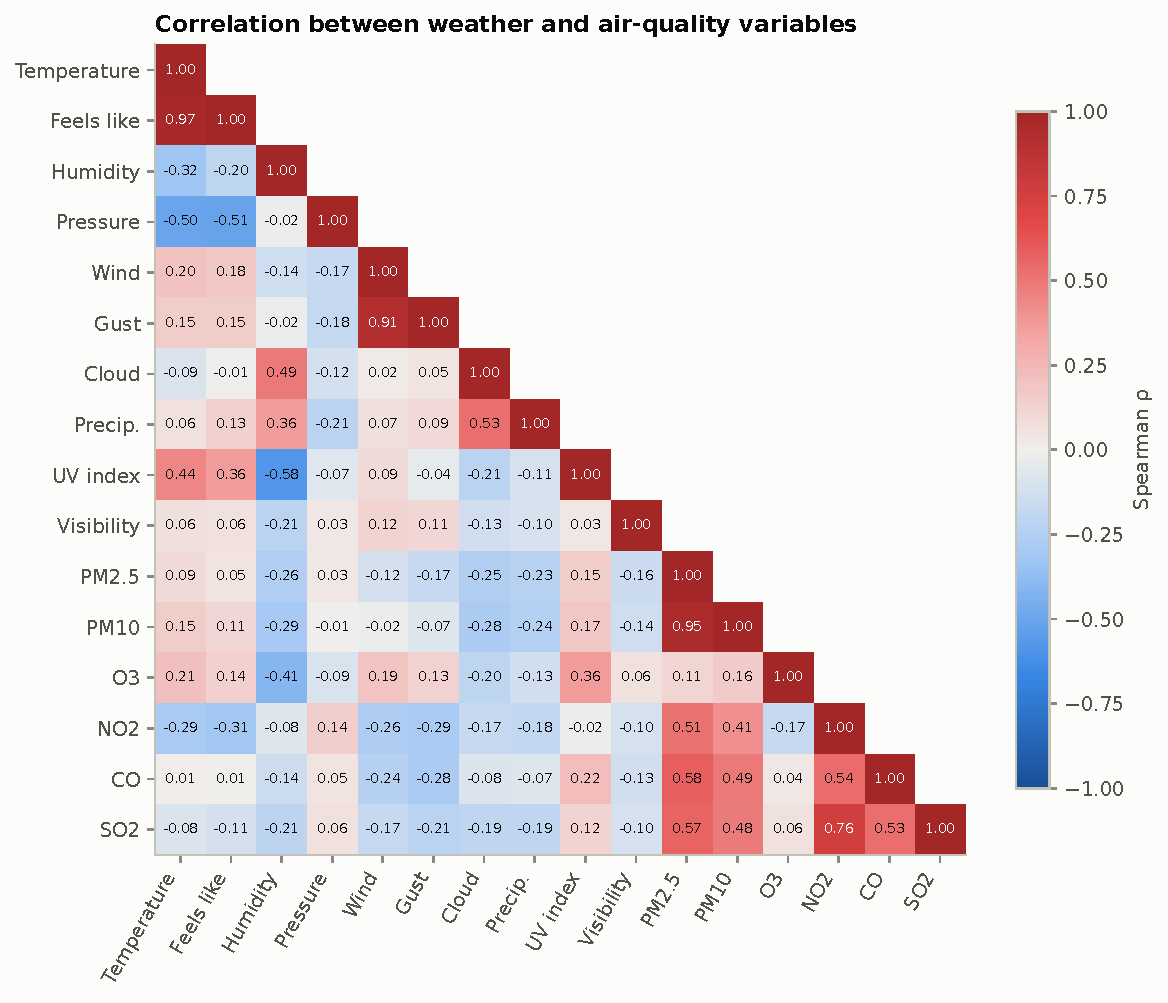
\includegraphics[width=0.72\linewidth]{eda/correlation_matrix}
\caption{Spearman correlation matrix of weather and air-quality variables.}\label{fig:corr}
\end{figure}
